In this exercise we implement UCB Q-learning in the 5-state RiverSwim environment. The algorithm is run with the parameters:
\[
\gamma = 0.92,\quad \varepsilon = 0.13,\quad \delta = 0.05,\quad T = 2\times10^6.
\]
The starting state is sampled uniformly and we set 
\[
H = \Big\lceil\frac{1}{1-\gamma}\log\frac{1}{\varepsilon}\Big\rceil,\quad b(k) = \sqrt{\frac{H}{k}\log\Big(SA\log(k+1)/\delta\Big)}.
\]
The performance is measured by the cumulative number of $\varepsilon$-bad steps,
\[
n(t)=\sum_{\tau=1}^{t}\mathbf{1}\{V^{\pi_\tau}(s_\tau) < V^*(s_\tau)-\varepsilon\},
\]
where $V^*(s)$ is computed via value iteration. In our experiments the value iteration procedure yields:
\[
V^* = [2.83439639,\; 3.45056954,\; 4.27771502,\; 5.31104628,\; 6.594788].
\]

Below is the complete implementation of the UCB Q-learning routine.

\begin{lstlisting}[caption={Complete UCB Q-learning routine}, label=lst:ucbql]
def run_ucb_ql(T, gamma, epsilon_eval, delta, H, V_star, record_interval=1000, seed=None):
    if seed is not None:
        np.random.seed(seed)
    env = riverswim(5)
    # Sample starting state uniformly.
    env.s = np.random.randint(0, env.nS)
    s = env.s
    S = env.nS
    A = env.nA
    R_max = 1.0
    optimistic_init = R_max / (1.0 - gamma)
    Q = np.full((S, A), optimistic_init)
    Q_hat = np.copy(Q)
    N = np.ones((S, A))
    n_bad = 0
    times = []
    n_values = []
    # Cache for policy evaluation
    policy_value_cache = {}
    for t in range(1, T + 1):
        # Select action greedily w.r.t. Q_hat.
        a = np.argmax(Q_hat[s, :])
        new_s, r = env.step(a)
        k = N[s, a]
        alpha_k = (H + 1) / (H + k)
        bonus = np.sqrt((H / k) * np.log(S * A * np.log(k + 1) / delta))
        # Q-update with exploration bonus.
        Q[s, a] = (1 - alpha_k) * Q[s, a] + alpha_k * (r + bonus + gamma * np.max(Q_hat[new_s, :]))
        Q_hat[s, a] = min(Q_hat[s, a], Q[s, a])
        N[s, a] += 1
        # Evaluate current greedy policy.
        policy = np.argmax(Q_hat, axis=1)
        policy_tuple = tuple(policy)
        if policy_tuple not in policy_value_cache:
            V_policy = evaluate_policy(policy, env, gamma)
            policy_value_cache[policy_tuple] = V_policy
        else:
            V_policy = policy_value_cache[policy_tuple]
        if V_policy[new_s] < V_star[new_s] - epsilon_eval:
            n_bad += 1
        s = new_s
        if t % record_interval == 0:
            times.append(t)
            n_values.append(n_bad)
    return np.array(times), np.array(n_values)
\end{lstlisting}

\subsection*{(i) Sample Path of $n(t)$}
A single run of the algorithm produces a sample path of the cumulative $\varepsilon$-bad steps $n(t)$. Figure~\ref{fig:sample_path} shows the sample path. This plot illustrates the steady accumulation of bad steps over time.

\begin{figure}[H]
  \centering
  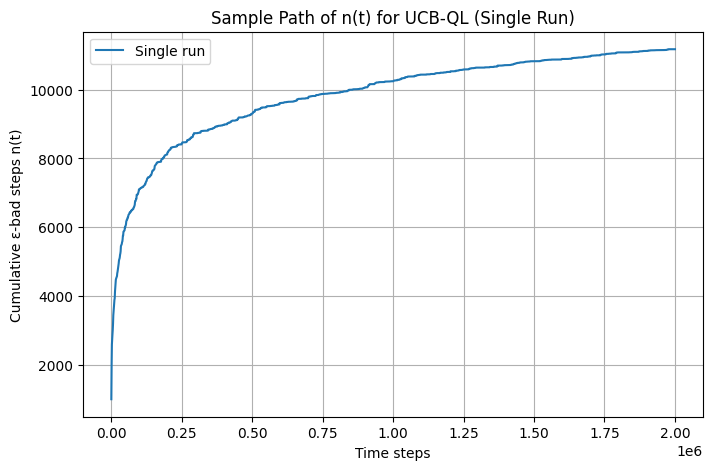
\includegraphics[width=0.8\textwidth]{Code/sample_path_ucbql.png} % Replace with your actual image file
  \caption{Sample path of the cumulative number of $\varepsilon$-bad steps $n(t)$ for a single run.}
  \label{fig:sample_path}
\end{figure}

\subsection*{(ii) Averaged $n(t)$ over 100 Runs}
In addition, the algorithm was executed over 100 independent runs. Figure~\ref{fig:avg_nt} shows the average $n(t)$ with 95\% confidence intervals. Notably, the individual runs exhibit very similar behavior, as evidenced by the tight confidence bounds.

\begin{figure}[H]
  \centering
  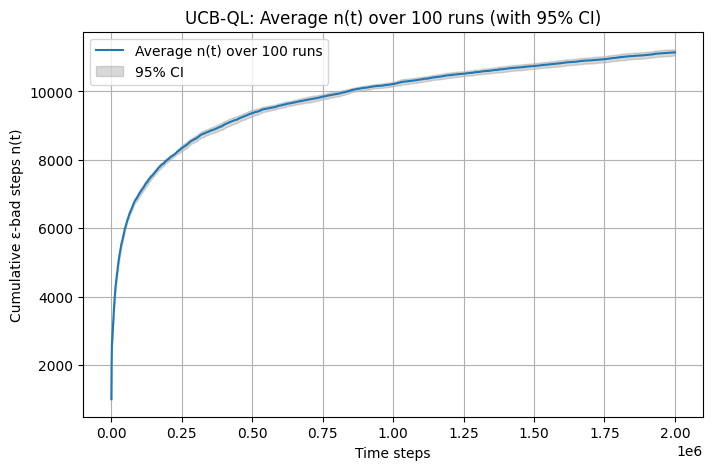
\includegraphics[width=0.8\textwidth]{Code/average_n_t_ucbql.png} % Replace with your actual image file
  \caption{Averaged $n(t)$ over 100 runs with 95\% confidence intervals.}
  \label{fig:avg_nt}
\end{figure}

In conclusion, the experimental results confirm that UCB Q-learning consistently maintains a similar behavior across runs, with the cumulative $\varepsilon$-bad steps growing as expected in the RiverSwim environment.